\documentclass{article}

\usepackage[a4paper, total={6in, 9in}]{geometry}
\usepackage[utf8]{inputenc}
\usepackage[ngerman]{babel}
\usepackage[hidelinks]{hyperref}
\usepackage{graphicx}
\usepackage{tabularx}
% \usepackage{showframe}
\usepackage[noframe]{showframe}
\usepackage{float}
\usepackage[style=ieee,backend=biber]{biblatex}
\addbibresource{bib/literature}
\usepackage{csquotes}
\emergencystretch=1em
\usepackage{fancyhdr}

% add and format date
\usepackage{datetime}
\newdateformat{monthdayyeardate}{%
  \THEDAY. \monthname[\THEMONTH] \THEYEAR}

% setup fancy header
\pagestyle{fancy}
\fancyhf{}
\rhead{Top right text}
\lhead{Top left text}
\rfoot{Seite \thepage}
\lfoot{\monthdayyeardate\today}

\begin{document}

\section{Example Section}\label{section_one}

Citation \cite{aharonov2008quantum}.

% add vertical space
\vspace{1cm}

Reference to \autoref{section_one}

\begin{figure}[H]
  \centering
  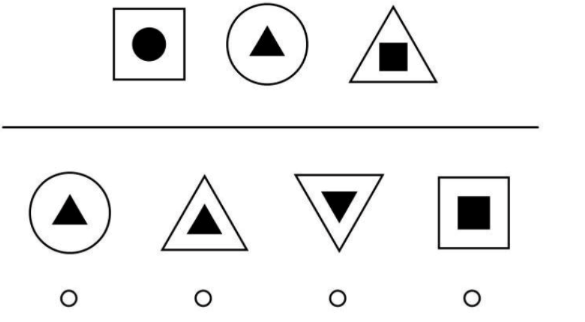
\includegraphics[scale=.5]{figures/example_figure.png} \\
  \caption{Example Figure}\label{fig:example_figure}
\end{figure}

\begin{table}[htbp]
  \centering
  \begin{tabularx}{\textwidth}{| p{1cm} | X | p{6cm} |}
    \hline
      1 & Lorem
        & Ipsum \\ \hline
      2 & Dolorum
        & Est \\ \hline
  \end{tabularx}
  \caption{Example Table}\label{tbl:example_table}
\end{table}

\begin{figure}[H]
  \[ E = m c^2 \]
  \caption{Example Equation}\label{eq:example_equation}
\end{figure}

% **************************************
% Table of figure/tables & bibliography
% **************************************
\listoffigures
\listoftables
\printbibliography
\end{document}
